% !TEX root =  ../main_manuscript.tex

\section{Results}
\label{sec:results}
We first discuss the results pertaining to the joint model fitted to the PRIAS dataset and then discuss results from the simulation study.
\subsection{Model Fit}
From the joint model fitted to the PRIAS dataset, we found that both $\log_2 \{\mbox{PSA} + 1\}$ velocity,  and log odds of having $\mbox{DRE} > \mbox{T1c}$  were significantly associated with the hazard of cancer progression. For any patient, an increase in $\log_2 \{\mbox{PSA} + 1\}$ velocity from −0.03 to 0.16 (first and third quartiles of the fitted velocities, respectively) corresponds to a 1.92 fold increase in the hazard of cancer progression. Whereas, an increase in log odds of $\mbox{DRE} > \mbox{T1c}$ from -6.65 to -4.36 (first and third quartiles of the fitted log odds, respectively) corresponds to a 1.40 fold increase in the hazard of cancer progression. In terms of the predictive performance, we found that the area under the receiver operating characteristic curves (AUC) \cite{landmarking2017} was 0.59, 0.66, and 0.66 at years 1, 2, and 3 of follow‐up, respectively. The AUC estimates for a joint model ignoring DRE measurements were 0.58, 0.64 and 0.60 at years 1, 2 and 3 of follow-up. Parameter estimates are presented in detail in Web Appendix C.

\subsection{Simulation Study}
In the 500$\times$750 training patients, we observed that for roughly 50\% of the patients cancer progression did not take place in the 10 year follow-up. These could be seen as patients with a slow speed of cancer progression. Roughly 30\% of the patients obtain cancer progression within first 3.5 years. These could be high risk patients who choose AS instead of immediate treatment, or patients with an initially misdiagnosed state of cancer \cite{cooperberg2011outcomes}. In this work we consider these patients as the fast progressing patients. We consider that the remaining 20\% patients with cancer progression times between 3.5 and 10 years have an intermediate speed of cancer progression.
\begin{figure}[!htb]
\captionsetup{justification=justified}
\centerline{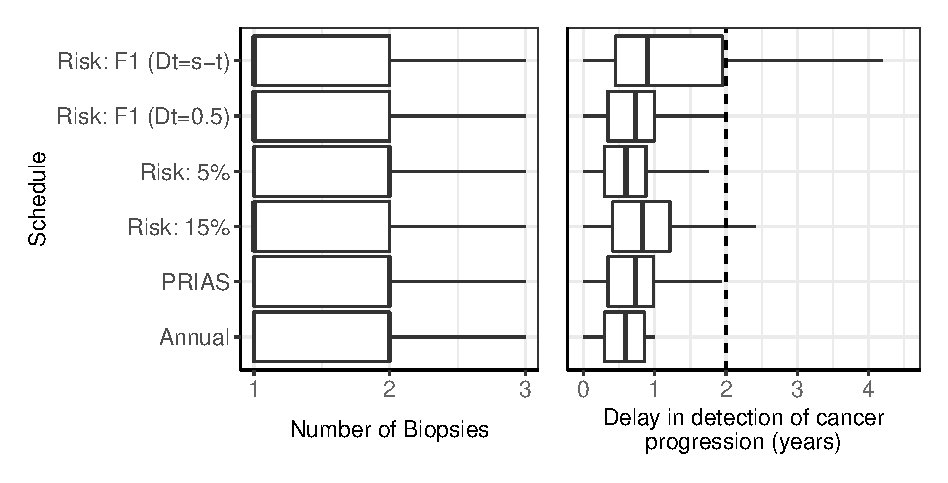
\includegraphics[width=\columnwidth]{images/sim_res_fast.eps}}
\caption{Boxplot showing variation in number of biopsies, and the delay in detection of cancer progression, in years (time of last biopsy - true time of cancer progression) for various biopsy schedules. The plot presents results for only those simulated test patients who had a faster speed of cancer progression, with progression times between 0 and 3.5 years. Biopsies are conducted until cancer progression is detected. Types of personalized schedules: Risk: 15\% and Risk: 5\% schedules, schedule biopsy if the risk of cancer progression at a visit is more than 15\% and 5\%, respectively. Risk: F1 (Dt=0.5) and Risk: F1 (Dt=s-t) work similar to Risk: 15\% and Risk: 5\%, except that the risk threshold for biopsy is chosen automatically by maximizing $\mbox{F}_1$ score. The term Dt represents the time window (years) in which $\mbox{F}_1$ score is maximized, and $s$ is the time of the current follow-up visit and $t$ is the time of the latest biopsy  Annual corresponds to a schedule of yearly biopsies and PRIAS corresponds to biopsies as per PRIAS protocol.}
\label{fig:sim_res_fast}
\end{figure}

For faster progressing patients (30\% of the total patients), the boxplot in Figure \ref{fig:sim_res_fast} shows the variation in number of biopsies, and the delay in detection of cancer progression, in years (time of last biopsy - true time of cancer progression) due to various biopsy schedules. We can see that the personalized schedules conduct a median of one biopsy compared to two biopsies for PRIAS and annual schedule. The performance of personalized schedule with automatically chosen threshold is similar to that of PRIAS schedule. Thus with personalized approach, one biopsy may get saved for faster progressing patients.
\begin{figure}[!htb]
\captionsetup{justification=justified}
\centerline{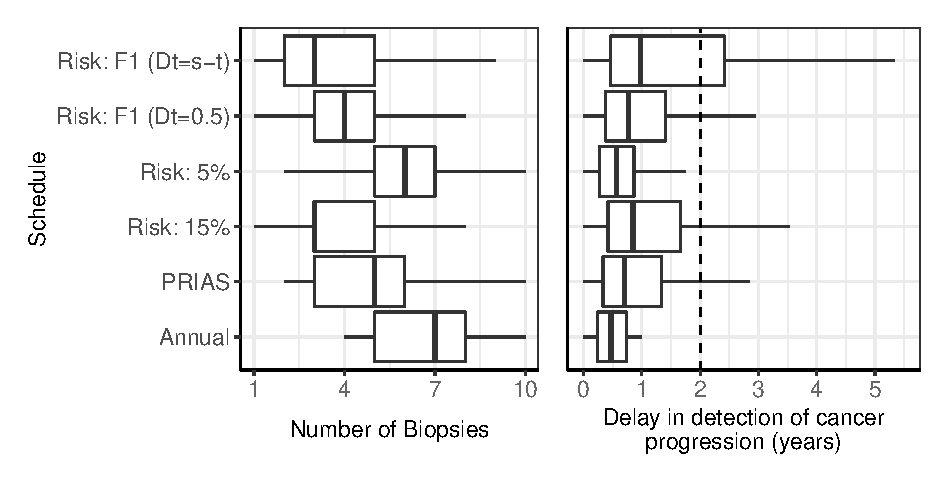
\includegraphics[width=\columnwidth]{images/sim_res_intermediate.eps}}
\caption{Boxplot showing variation in number of biopsies, and the delay in detection of cancer progression, in years (time of last biopsy - true time of cancer progression) for various biopsy schedules. The plot presents results for only those simulated test patients who had an intermediate speed of cancer progression, with progression times between 3.5 and 10 years. Biopsies are conducted until cancer progression is detected. Types of personalized schedules: Risk: 15\% and Risk: 5\% schedules, schedule biopsy if the risk of cancer progression at a visit is more than 15\% and 5\%, respectively. Risk: F1 (Dt=0.5) and Risk: F1 (Dt=s-t) work similar to Risk: 15\% and Risk: 5\%, except that the risk threshold for biopsy is chosen automatically by maximizing $\mbox{F}_1$ score. The term Dt represents the time window (years) in which $\mbox{F}_1$ score is maximized, and $s$ is the time of the current follow-up visit and $t$ is the time of the latest biopsy  Annual corresponds to a schedule of yearly biopsies and PRIAS corresponds to biopsies as per PRIAS protocol.}
\label{fig:sim_res_intermediate}
\end{figure}

For patients with intermediate progression speed (20\% of the total patients), the boxplot in Figure \ref{fig:sim_res_intermediate} shows the variation in number of biopsies, and the delay in detection of cancer progression due to various biopsy schedules. Firstly, we can see that personalized schedules with a small risk threshold such as 5\% risk conduct many more biopsies than other personalized schedules. Consequently, their performance with respect to the delay in detection of progression is similar to that of annual schedule. However, personalized schedule with slightly higher risk (15\%) and risk chosen automatically, schedule a median of 3 and 4 biopsies, respectively. This is despite the fact that the delay in detection of cancer progression due to these schedules is similar to that of PRIAS. The PRIAS schedule also conducts more biopsies (median of 5 biopsies). Thus, personalized approach may lead to one to two less biopsies for patients with intermediate speed of progression.

\begin{figure}[!htb]
\captionsetup{justification=justified}
\centerline{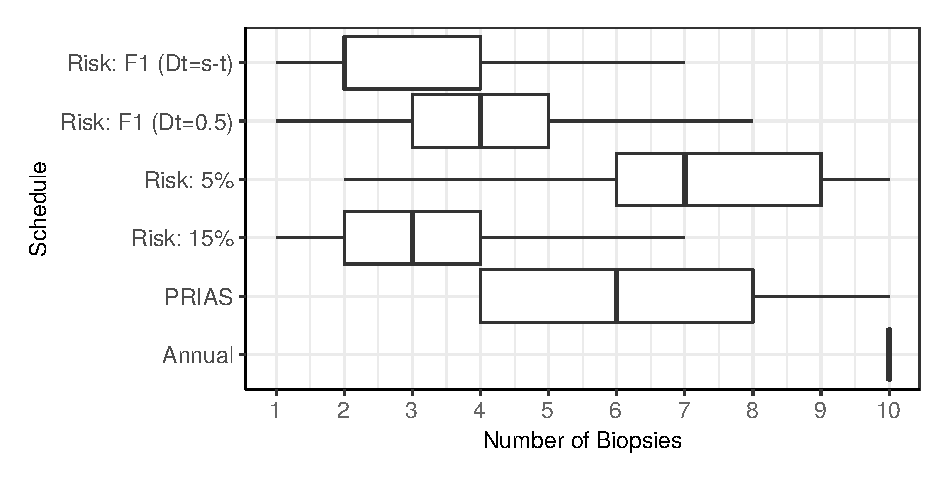
\includegraphics[width=\columnwidth]{images/sim_res_slow.eps}}
\caption{Boxplot showing variation in number of biopsies conducted by various biopsy schedules for those simulated test patients who did not have cancer progression over a period of 10 years. Biopsies are conducted until cancer progression is detected. Types of personalized schedules: Risk: 15\% and Risk: 5\% schedules, schedule biopsy if the risk of cancer progression at a visit is more than 15\% and 5\%, respectively. Risk: F1 (Dt=0.5) and Risk: F1 (Dt=s-t) work similar to Risk: 15\% and Risk: 5\%, except that the risk threshold for biopsy is chosen automatically by maximizing $\mbox{F}_1$ score. The term Dt represents the time window (years) in which $\mbox{F}_1$ score is maximized, and $s$ is the time of the current follow-up visit and $t$ is the time of the latest biopsy  Annual corresponds to a schedule of yearly biopsies and PRIAS corresponds to biopsies as per PRIAS protocol.}
\label{fig:sim_res_slow}
\end{figure}

The patients who are at most advantage with personalized schedules are the patients who progress slowly (50\% of the total patients). Figure \ref{fig:sim_res_slow} shows a boxplot of the number of biopsies conducted by various biopsy schedules for such patients. It can be seen that the annual schedule may lead to 10 unnecessary biopsies for everyone. The PRIAS schedule, schedules a median of 6 unnecessary biopsies. In comparison the personalized schedules using 15\% and automatically chosen risk schedule only 3 and 4 biopsies, respectively.